% !TEX root = ../thesis.tex

\chapter{研究方法与设计 (Research Methodology and Design)} \label{chp:methodology}

\section{总体研究设计与技术路线}

本研究采用系统性、递进式的研究设计,旨在系统性地回答三个核心研究问题,并通过技术创新、方法学贡献和实证验证,构建一个完整的解决方案。研究的总体技术路线体现了从理论构建到技术实现,再到临床验证和应用转化的完整链条,确保每个研究环节都有明确的目标、科学的方法和可衡量的成果。

\begin{figure}[htbp]
\centering
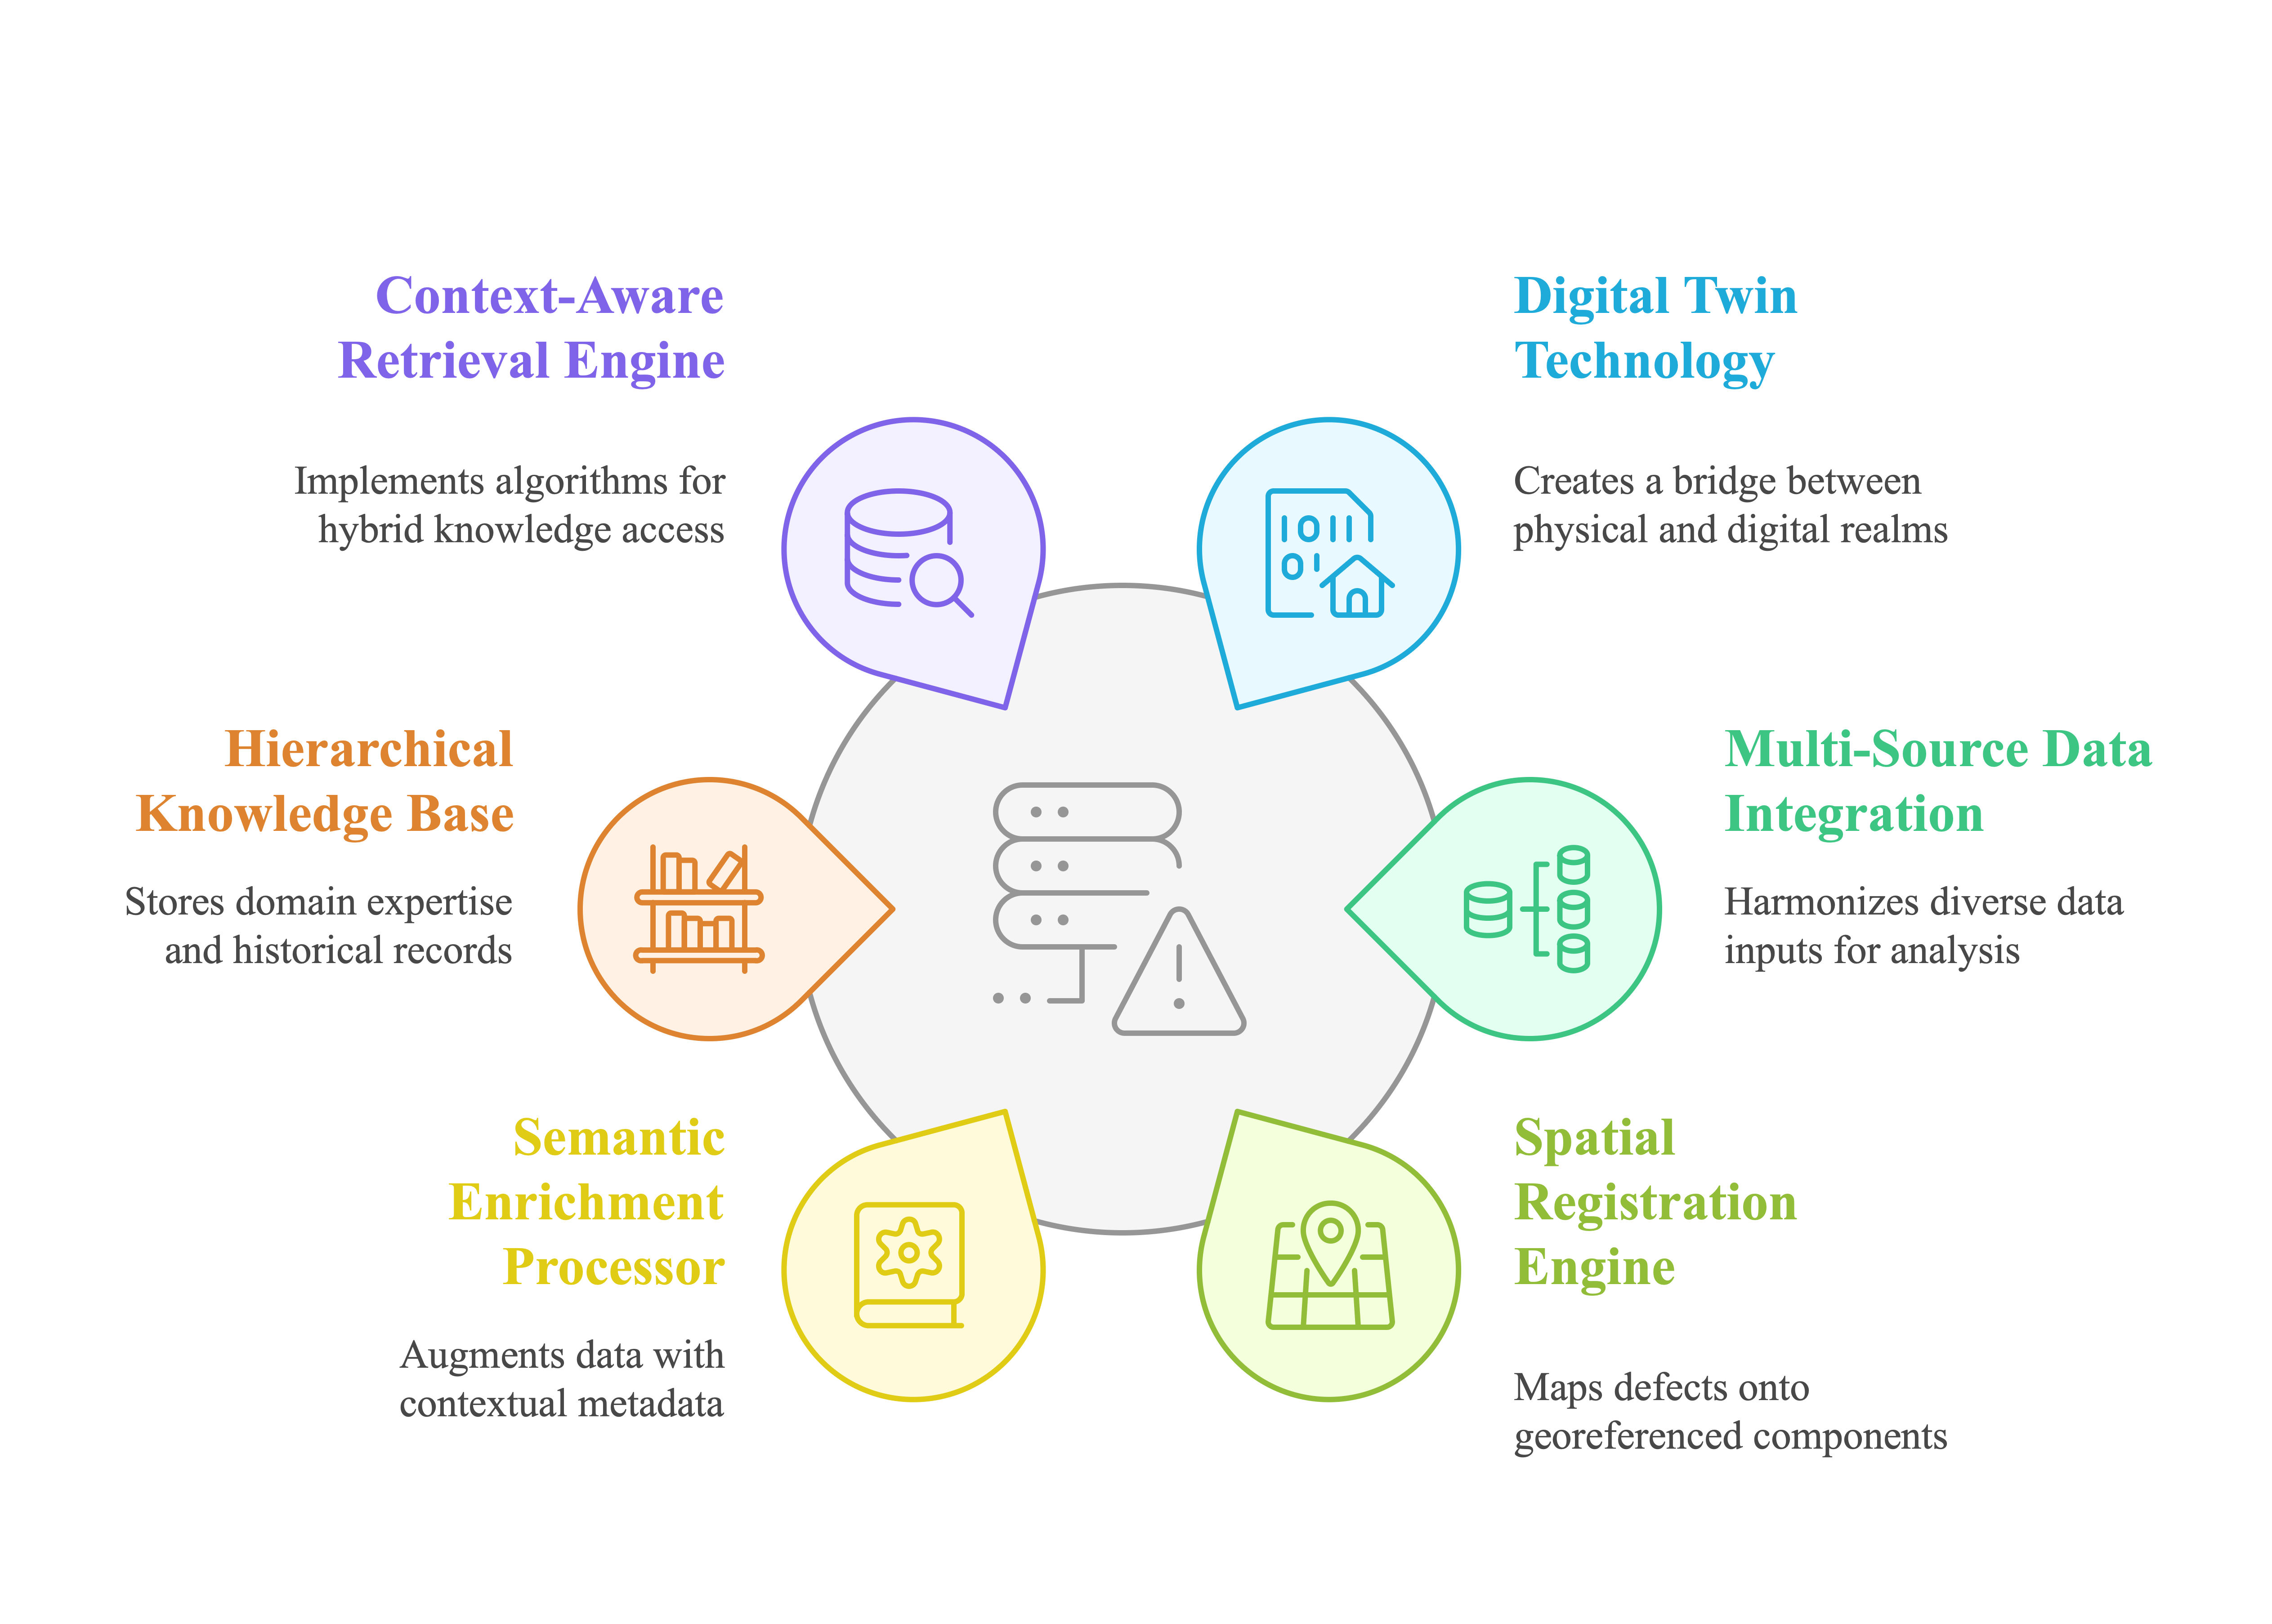
\includegraphics[width=0.9\textwidth]{DefectGPT/Overall_Framework.png}
\caption{总体技术路线图,展示了三个研究问题、研究目标与具体研究内容之间的逻辑关系}
\label{fig:overall_framework}
\end{figure}

技术路线的设计遵循"问题导向-解决方案-验证评估"的科学研究范式。针对RQ1(统一计算框架的构建问题),研究将从理论分析出发,基于"四大协同支柱"理论,设计并实现USANet统一框架,通过"两阶段知识注入"训练策略,实现胃癌和胰腺癌评估任务的协同学习。针对RQ2(临床信任的价值验证问题),研究将建立超越传统技术指标的多维度验证体系,通过技术性能、临床终点关联和决策价值三个层面的综合评估,确保AI框架的临床价值得到科学、严谨的验证。

针对RQ3(临床工作流的无缝整合问题),研究将设计并开发Sono-Agent人机协同工作流原型,通过实时动态扫查辅助和知识增强的智能报告生成,探索AI技术在超声诊断工作流中的深度整合。整个研究设计强调理论与实践的结合、技术创新与临床需求的对接,确保研究成果既有学术价值,又有实际应用前景。

\section{数据集的构建与伦理考量}

\subsection{数据来源与收集标准(多中心回顾性数据)}

本研究将构建一个高质量、大规模的多中心胃癌与胰腺癌经腹超声数据集,这是实现统一框架训练和验证的基础。数据收集将采用多中心回顾性研究设计,计划与国内外5-8家具有丰富超声诊断经验的三甲医院合作,包括消化内科、肿瘤科、超声科等多个科室。这种多中心设计能够确保数据的代表性和多样性,有效减少单中心数据可能存在的偏倚,提升模型的泛化能力。

数据收集的时间窗口设定为2018年1月至2023年12月,这一时间段能够确保数据的时效性,同时积累足够的病例数量。收集标准将严格遵循医学研究的伦理规范和数据质量要求,确保所有数据的合法性、准确性和完整性。参与的医疗机构将根据其病例数量、技术水平和数据质量进行严格筛选,确保数据集的整体质量。

\subsection{胃癌数据集:纳入与排除标准、样本量、影像类型}

胃癌数据集的构建将遵循严格的纳入与排除标准。纳入标准包括:(1) 年龄18-80岁的患者;(2) 经病理确诊的胃癌患者或经长期随访(≥2年)确认的良性病变患者;(3) 具有完整的经腹超声检查记录,包括静态图像和动态视频;(4) 超声检查与病理诊断间隔不超过30天;(5) 临床资料完整,包括TNM分期、治疗方案和随访结果。

排除标准包括:(1) 图像质量过差,无法进行有效评估;(2) 合并其他腹部恶性肿瘤;(3) 术前已接受新辅助化疗或放疗;(4) 临床资料不完整或随访丢失。基于初步调研和样本量计算,胃癌数据集目标收集病例数为2000-3000例,其中恶性病例占60-70\%,良性病例占30-40\%。影像类型将包括标准化的静态图像(DICOM格式)和动态扫查视频(MP4或AVI格式),每个病例至少包含10-15张关键静态图像和2-3段动态视频。

\subsection{胰腺癌数据集:纳入与排除标准、样本量、影像类型}

胰腺癌数据集的纳入标准与胃癌类似,但会特别关注胰腺癌的特殊性。纳入标准包括:(1) 年龄18-85岁的患者;(2) 经病理确诊的胰腺癌患者或经影像学和临床随访确认的良性胰腺病变;(3) 经腹超声能够清晰显示胰腺,图像质量满足评估要求;(4) 具有完整的CT或MRI对照资料;(5) 临床分期和治疗信息完整。考虑到胰腺癌的相对稀少性和经腹超声观察胰腺的技术难度,胰腺癌数据集的收集将更加注重质量控制。

排除标准除了与胃癌数据集类似的条件外,还包括:(1) 胰腺显示不清或完全被肠气遮挡;(2) 慢性胰腺炎等严重影响胰腺形态的良性疾病;(3) 胰腺内分泌肿瘤等特殊类型肿瘤。目标收集胰腺癌数据集1500-2500例,恶性与良性比例约为5:5。由于胰腺超声检查的特殊性,将特别收集不同体位(仰卧位、侧卧位)和不同饮水状态(空腹、饮水后)的图像,以最大化胰腺的可视化效果。

\subsection{数据标注:多名资深医师交叉标注与审核}

数据标注是确保数据集质量的关键环节,本研究将建立严格的多级标注和质控体系。标注团队将由来自不同医院的10-15名具有10年以上超声诊断经验的副主任医师及以上级别的专家组成,其中包括专门从事消化系统超声诊断的专家。标注工作将分为三个层次:初级标注、交叉审核和专家终审。

标注内容将包括:(1) 病灶边界框标注,使用标准的矩形框标记可疑病灶的位置和范围;(2) 精确分割掩码,对于明确的病灶进行像素级的分割标注;(3) 良恶性分类标注,基于形态学特征给出良恶性的概率评估;(4) 关键影像特征标注,包括回声特点、边界特征、血流信号、与周围结构的关系等临床诊断要素。每个病例将由至少3名不同医师独立标注,标注结果的一致性将通过Kappa值进行量化评估,对于一致性较低的病例将组织专家会诊确定最终标注。

\subsection{数据匿名化与伦理审批}

数据隐私保护和伦理合规是本研究的重要组成部分。所有收集的医学数据将严格按照《个人信息保护法》、《数据安全法》等相关法律法规进行处理。数据匿名化过程将包括:(1) 移除所有直接身份识别信息,如姓名、身份证号、联系方式等;(2) 对间接身份识别信息进行去标识化处理,如出生日期替换为年龄区间、地址替换为地区代码等;(3) 对影像数据进行技术处理,移除可能包含患者信息的DICOM标签。

本研究将在开始数据收集前,向各参与医院的伦理委员会提交详细的研究方案,申请伦理审批。伦理审批将涵盖研究的科学性、必要性、风险评估、数据使用范围、数据安全措施等方面。对于回顾性研究,将申请免除知情同意的伦理豁免,但会建立严格的数据使用监督机制。此外,还将建立数据安全管理制度,包括数据访问权限控制、数据传输加密、数据存储安全等措施,确保患者隐私得到充分保护。

\section{研究内容一:统一计算框架的构建 (回答RQ1)}

\subsection{理论基础:基于多任务学习与表征解耦的协同学习}

本研究构建统一框架的理论基础,源于机器学习领域的两大核心思想:多任务学习(Multi-Task Learning, MTL)和表征学习(Representation Learning)。MTL的核心思想是,通过让一个模型同时学习多个相关的任务,可以利用任务之间的共性信息,使得模型学习到的特征表征更具泛化性,从而提升在每个单一任务上的性能。这与本研究的"四大协同支柱"理论高度契合,胃癌和胰腺癌的评估任务,正是这样一组存在内在关联的"相关任务"。

然而,简单地共享一个编码器进行多任务学习,可能会导致任务间的"负迁移"或梯度冲突问题。因此,本研究将进一步引入表征解耦(Representation Disentanglement)的思想。其目标是让模型学习到的特征向量中,不同的部分对应于不同的、可解释的变异来源。例如,一部分特征可能编码了器官的通用解剖结构(任务共享信息),而另一部分特征则编码了特定病灶的属性(任务独有信息)。通过这种方式,我们旨在最大化任务间的正向协同,同时最小化任务间的相互干扰,从而实现更高效、更鲁棒的协同学习。

\subsection{核心方法:"两阶段知识注入(Two-Stage Knowledge Injection)"训练策略}

为了将上述理论转化为一个实际可行的训练流程,本研究设计了一种新颖的"两阶段知识注入"训练策略。这一策略的核心在于,模仿人类医生的学习过程——先学习通用的解剖学知识,再学习具体的疾病诊断知识。

第一阶段,通用腹部表征预训练:在这个阶段,我们并不需要大量精细标注的癌症数据。相反,我们将利用多中心收集的、更大规模的、仅有粗略标注(例如,仅知道这是上腹部扫查)甚至完全无标注的腹部超声视频数据。通过自监督学习(Self-Supervised Learning)的方法,如对比学习(MoCo, SimCLR)或掩码图像建模(MAE),我们强迫模型去学习腹部超声影像中通用的、内在的视觉规律和解剖结构。这一阶段的产物,是一个强大的视觉编码器(Encoder),它如同一个已经学习了《解剖学》的学生,对腹部的基本"语法"有了深刻理解。

第二阶段,多任务知识联合微调:在这个阶段,我们将"冻结"或以较小的学习率"微调"在第一阶段预训练好的编码器,并在其之上加载为胃癌和胰腺癌评估任务专门设计的多个任务头(Task-specific Heads)。然后,我们使用高质量、精标注的胃癌与胰腺癌数据集,对这些任务头以及(可选地)编码器的上层进行联合训练。这一过程,相当于让已经懂了解剖学的学生,开始学习《肿瘤诊断学》。由于编码器已经具备了强大的通用表征能力,第二阶段的微调过程将变得更高效、更稳定,并且能更好地利用宝贵的、带有金标准标注的数据,从而将特定于疾病的诊断知识,精准地"注入"到模型中。

\subsection{模型架构:Unified Sonographic Assessment Network (USANet)}

USANet(Unified Sonographic Assessment Network)是本研究提出的统一深度学习框架的核心技术实现。该网络的设计充分考虑了超声图像的特殊性质和多任务学习的要求,采用了先进的混合架构设计。

\textbf{Backbone设计}:USANet的主干网络选用先进的CNN-Transformer混合架构,具体采用ConvNeXt或MaxViT作为编码器。这种设计能够兼顾局部纹理特征提取和全局上下文建模能力。CNN组件负责提取超声图像中的细节纹理信息,对于识别病灶的微细特征(如回声模式、边界特征等)至关重要。Transformer组件则通过自注意力机制捕捉全局的解剖关系,能够有效建模胃和胰腺之间的空间关系以及病灶与周围结构的相互作用。

\textbf{Task Heads设计}:在统一的编码器之上,USANet设计了四个专门的任务头,分别处理不同的评估任务:

(1) 定位头(Localization Head):基于类似YOLO或DETR的结构,输出病灶的边界框。该模块能够同时检测胃部和胰腺的可疑病灶,并给出精确的位置信息。

(2) 分割头(Segmentation Head):基于类似U-Net的结构,输出像素级的分割掩码。该模块能够对检测到的病灶进行精确的轮廓勾画,为后续的形态学分析提供基础。

(3) 分类头(Classification Head):对编码后的特征进行全局平均池化,通过全连接层输出良恶性概率。该模块整合全图信息,给出整体的诊断判断。

(4) 属性评估头(Attribute Assessment Head):多个并行的分类/回归头,用于评估与TNM分期强相关的影像特征。例如,针对胃癌评估浆膜侵犯的迹象,针对胰腺癌评估血管包裹的关系等。

\subsection{损失函数设计}

为了有效训练多任务网络,本研究设计了一个加权的复合损失函数:

$$L_{total} = w_1 L_{loc} + w_2 L_{seg} + w_3 L_{cls} + w_4 L_{attr}$$

其中,$L_{loc}$为定位损失,采用Focal Loss或GIoU Loss来处理目标检测中的类别不平衡问题;$L_{seg}$为分割损失,使用Dice Loss和Cross-Entropy Loss的组合;$L_{cls}$为分类损失,采用加权的Cross-Entropy Loss处理良恶性样本不平衡;$L_{attr}$为属性评估损失,根据具体属性的性质选择适当的损失函数。

权重$w_1, w_2, w_3, w_4$的设置将通过实验确定,并研究动态权重调整策略,如使用不确定性加权(Uncertainty Weighting)或梯度归一化(GradNorm)等方法来平衡不同任务的学习进程,避免某个任务主导整个训练过程。

\subsection{实验设置与对比实验}

为了全面评估USANet的性能,本研究将设计严格的对比实验。对比基线将包括:(1) 多个"单一任务,单一模型"的专用网络,分别针对胃癌检测、胰腺癌检测、良恶性分类等任务进行训练;(2) 简单的多任务网络,不使用"两阶段知识注入"策略;(3) 现有的医学影像分析网络,如在医学影像领域广泛使用的ResNet、DenseNet等。

消融实验(Ablation Study)将系统性地验证各个组件的有效性:(1) 验证"两阶段训练策略"的有效性,通过与端到端训练进行对比;(2) 验证"多任务联合学习"的优势,通过与单任务学习进行对比;(3) 验证不同架构组件的贡献,如CNN vs. Transformer,不同的注意力机制等;(4) 验证损失函数设计的合理性,通过不同权重设置和损失函数组合进行对比。

\section{研究内容二:多维度综合验证体系的建立 (回答RQ2)}

\subsection{技术性能验证 (Technical Validation)}

技术性能验证构成了AI模型评估的基础层面,旨在全面评估USANet在各个具体任务上的技术指标表现。验证将在独立的测试集上进行,该测试集来自于与训练集不同的医疗机构,以确保评估的客观性和泛化性。

针对分类任务,将评估以下关键指标:准确率(Accuracy)反映整体诊断正确率;精确率(Precision)和召回率(Recall)分别评估模型对阳性病例的识别能力和覆盖能力;F1分数提供精确率和召回率的调和平均值;AUC值(Area Under the ROC Curve)评估模型在不同阈值下的综合性能,并绘制详细的ROC曲线进行可视化分析。特别地,我们将使用DeLong检验来比较不同模型间的AUC差异是否具有统计学意义,确保性能提升的统计学可靠性。

针对分割任务,将采用医学图像分割领域的标准指标:Dice系数(Dice Coefficient)衡量预测分割与真实分割的重叠程度;IoU(Intersection over Union)评估预测区域与真实区域的交并比;Hausdorff距离评估分割边界的精确性;平均表面距离(Average Surface Distance)提供更细致的边界质量评估。

针对定位任务,将使用目标检测领域的经典指标:mAP(mean Average Precision)在不同IoU阈值下评估检测性能;精确率-召回率曲线评估检测器在不同置信度阈值下的表现;漏检率和误检率分析模型的稳定性和可靠性。

\subsection{临床终点关联验证 (Clinical Endpoint Correlation)}

临床终点关联验证是本研究验证体系的核心创新,旨在建立AI模型输出与最权威临床标准之间的直接关联。这一验证超越了传统的影像标注比较,直接链接到患者的最终诊断和预后信息。

\textbf{金标准建立}:本研究将系统性收集测试集患者的术后病理诊断报告、TNM分期信息、治疗方案选择和长期随访结果。病理诊断报告将由病理科专家进行标准化解读和编码,TNM分期将按照最新的国际肿瘤分期标准进行统一分类,随访信息将包括治疗反应、复发情况、生存状态等关键终点。

\textbf{关联分析I(定性诊断)}:验证模型的良恶性判断与病理结果的一致性。分析将采用多种统计方法:Kappa值评估诊断一致性的强度;混淆矩阵分析错误诊断的模式和原因;分层分析不同亚组(如不同年龄、性别、病理类型)中的诊断一致性;敏感性分析评估模型在不同病理类型中的表现差异。

\textbf{关联分析II(分期评估)}:验证模型输出的关键影像特征评估结果与病理T分期、N分期之间的相关性。使用Spearman等级相关分析评估影像特征与病理分期的相关强度;采用ROC分析评估影像特征预测特定分期的能力;建立影像-病理对照表,分析不同影像表现对应的病理改变;进行多变量回归分析,识别最具预测价值的影像特征组合。

\subsection{临床决策价值验证 (Decision-Making Value)}

临床决策价值验证代表了本研究验证体系的最高层次,旨在量化AI框架在实际临床决策中的真实价值和净获益。这一验证直接回答"AI能否帮助医生做出更好的决策"这一根本问题。

\textbf{决策曲线分析 (Decision Curve Analysis, DCA)}:DCA是本验证的核心方法,通过绘制决策曲线来比较不同决策策略的临床净获益。具体实施包括:定义决策场景,如是否进行进一步检查、是否建议手术等关键临床决策点;设定风险阈值范围,通常为0.05到0.95,覆盖不同的临床偏好;计算净获益,考虑真阳性带来的益处和假阳性造成的损害;比较策略包括"仅医生诊断"、"AI模型辅助诊断"和"仅AI模型诊断"三种策略。

DCA分析将特别关注以下几个关键问题:在什么风险阈值范围内,AI辅助诊断能够提供最大的净获益?AI辅助能够帮助避免多少不必要的手术或漏诊?在不同的临床场景下(如筛查vs确诊),AI的价值如何变化?不同经验水平的医生使用AI辅助的获益是否不同?

\textbf{临床影响评估}:除了DCA分析外,研究还将评估AI框架对临床决策流程的具体影响,包括:诊断信心度的变化,通过问卷调查评估医生在使用AI辅助前后的诊断信心;决策时间的变化,测量AI辅助对诊断效率的影响;诊断一致性的改善,评估AI是否能够减少不同医生间的诊断差异;下游检查需求的变化,分析AI辅助是否能够优化后续的检查流程。

\section{研究内容三:人机协同工作流原型的探索 (回答RQ3)}

\subsection{原型名称与设计哲学:Sono-Agent}

Sono-Agent是本研究提出的人机协同工作流原型,其命名体现了"超声"(Sonography)与"智能代理"(Intelligent Agent)的结合。该原型的设计哲学基于三个核心原则:上下文感知(Context-Aware)、非干扰性(Non-Intrusive)、可信赖(Trustworthy)。

\textbf{上下文感知}意味着Sono-Agent能够理解当前的检查情境,包括患者的基本信息、检查目的、已有的临床发现等,并据此调整其辅助策略和建议内容。系统不是简单地分析孤立的图像,而是将每一帧图像、每一次测量都置于完整的检查上下文中进行理解。

\textbf{非干扰性}确保系统的智能辅助不会中断或干扰医生的正常检查流程。AI的建议和提示以低调、非强制的方式呈现,医生可以选择接受、忽略或进一步探索。系统的存在应该像一个默默工作的助手,在需要时提供帮助,在不需要时保持安静。

\textbf{可信赖性}要求系统的每个建议都有可追溯的依据,每个生成的内容都经过严格的事实核查。系统会明确区分高置信度和低置信度的建议,对于不确定的情况会坦诚地表达不确定性,避免过度自信可能带来的误导。

\subsection{模块一:实时动态扫查辅助 (Real-time Scan Assistance)}

实时动态扫查辅助模块是Sono-Agent的核心功能,旨在在超声检查进行过程中提供智能、实时的辅助信息。该模块的技术实现包括多个层面的创新。

\textbf{模型轻量化与优化}:为了实现实时处理,USANet模型将进行专门的轻量化处理。采用知识蒸馏技术将大模型的知识压缩到更小的网络中;使用TensorRT、ONNX等推理优化框架进行加速;设计专门的边缘计算版本,能够在连接超声设备的边缘设备上高效运行;实现动态批处理和帧率自适应,根据硬件性能自动调整处理频率。

\textbf{智能交互界面设计}:交互界面的设计遵循医学界面设计的最佳实践。可疑区域提示采用半透明热力图或闪烁边界框的形式,以低调的方式引起注意而不遮挡重要信息;置信度指示通过颜色深浅或边界粗细来表示AI建议的可信程度;上下文信息窗口在不占用主要视野的前提下,显示相关的诊断信息和建议;自适应显示根据检查阶段和发现自动调整界面布局和信息密度。

\textbf{智能引导策略}:系统能够基于当前的扫查情况提供智能的检查建议。扫查路径优化根据已检查的区域和发现,建议最优的下一步扫查方向;视角调整提示当发现可疑区域时,建议最佳的观察角度和探头位置;测量引导对于检测到的病灶,自动建议需要测量的参数和标准测量方法;动态跟踪对移动的病灶或因呼吸运动模糊的结构进行实时跟踪和稳定显示。

\subsection{模块二:知识增强的智能报告生成 (Knowledge-Augmented Smart Reporting)}

智能报告生成模块旨在检查结束后,自动整合检查过程中的关键发现,生成结构化、专业化的超声报告草稿。该模块的创新之处在于引入了知识增强机制,确保生成内容的准确性和可靠性。

\textbf{数据整合与结构化}:系统自动收集和整合检查过程中的所有关键信息,包括:关键阳性/可疑切面的自动捕获和归档;重要测量数据的自动记录和标准化;USANet评估结果的结构化存储;检查过程中医生的语音备注或文字注释;与患者相关的背景信息和既往检查对比。

这些异构数据将被整合到一个统一的结构化模板中,模板设计遵循医学报告的标准格式,包括患者基本信息、检查方法、主要发现、测量数据、诊断意见等标准章节。

\textbf{知识增强生成机制}:为了解决生成式AI的"幻觉"问题,本研究设计了创新的知识增强机制。医学知识图谱构建包含超声诊断领域的标准术语、诊断标准、正常值范围等权威知识;事实核查引擎对生成的每一句描述进行实时核查,确保内容有据可查;溯源机制为每个生成的结论提供明确的依据,要么来源于图像发现,要么来源于医学知识;不确定性表达对于模棱两可的发现,系统会明确表达不确定性而非强行给出结论。

\textbf{报告质量控制}:生成的报告将经过多层质量控制。语言质量检查确保医学术语使用准确、语法正确、表达清晰;内容逻辑性验证检查报告的内在逻辑一致性,避免自相矛盾的描述;标准符合性审查确保报告格式和内容符合医院和专业学会的标准;人工审核接口为医生提供便捷的修改和完善功能,支持快速编辑和个性化调整。

\subsection{可用性评估 (Usability Study)}

为了全面评估Sono-Agent原型的实用性和接受度,本研究将设计综合性的可用性研究。研究设计将采用定量和定性相结合的方法,确保评估的全面性和客观性。

\textbf{用户研究设计}:研究将邀请来自不同医院、不同年资的超声医生参与。参与者分组包括:>10年经验的专家组(15-20人),代表资深超声医生;<3年经验的初级组(15-20人),代表年轻医生;5-10年经验的中级组(10-15人),作为对照。每组医生将在模拟临床场景中使用Sono-Agent原型完成标准化的超声检查任务。

\textbf{评估指标体系}:可用性评估将采用多维度指标体系。系统可用性量表(System Usability Scale, SUS)提供标准化的可用性评分;任务完成时间测量AI辅助对检查效率的影响;诊断准确率变化评估AI辅助对诊断质量的影响;用户满意度通过李克特量表评估医生对系统各功能的满意程度;学习曲线分析不同年资医生掌握系统的难易程度。

\textbf{定性研究}:除定量指标外,研究还将包括深入的定性分析。半结构化访谈探索医生对AI辅助的深层态度和期望;焦点小组讨论收集改进建议和功能需求;行为观察记录医生与系统交互的自然行为模式;关键事件分析识别系统使用中的关键成功因素和障碍。

\textbf{迭代改进机制}:基于可用性研究的结果,建立系统迭代改进机制。快速原型修正根据用户反馈及时调整界面设计和交互逻辑;功能优先级排序基于用户需求确定后续开发重点;个性化定制探索为不同类型用户提供定制化界面的可能性;培训方案设计基于学习曲线分析设计有效的用户培训方案。

